\documentclass[12pt,english]{article}
\usepackage[a4paper,top=5mm, bottom=15mm]{geometry}
%\usepackage[parfill]{parskip}    % Activate to begin paragraphs with an empty line rather than an indent
\usepackage{graphicx}
\usepackage{amssymb}
\usepackage{amsmath}
\usepackage[numbers]{natbib}
\usepackage{booktabs}
\usepackage{subcaption}
\usepackage[capitalise]{cleveref}
% \usepackage[none]{hyphenat}
% \DeclareGraphicsRule{.tif}{png}{.png}{`convert #1 `dirname #1`/`basename #1 .tif`.png}

\usepackage{graphicx}
\graphicspath{{./figures/}}
\DeclareGraphicsExtensions{.pdf,.jpeg,.png,.jpg}

\newcommand{\ie}{i.e.,}
\newcommand{\eg}{e.g.,}
\newcommand*{\hurl}[1]{\href{http://#1}{\emph{#1}}}
\let\biconditional\leftrightarrow%

\pagestyle{empty}

\title{Solving the Banana Navigation Problem through Deep Reinforcement Learning}
\author{Alessandro Leite}

\date{}

\pagenumbering{gobble}

\begin{document}
\maketitle
\thispagestyle{plain}
\vspace{-60pt}

\section{Context}\label{sec:introduction}

An important concept in machine learning comprises the tasks of deciding from experience the sequence of action to perform in an uncertain environment to achieve some objective~\cite{francois:18}. Inspired by behavioral psychology~\cite{sutton:18}, reinforcement learning~(RL) proposes a formal framework in which an agent learns by iterating with an environment. Based on experiences gathered by this iteration, the agent learns to optimize some objectives represented in the form of cumulative rewards. Thus, reinforcement learning focuses on the problem of learning a behavioral policy, a mapping from states to actions, which maximizes cumulative long-term rewards~\cite{sutton:18}. A policy can be represented as a lookup table, listing the appropriate action from any state. Therefore, in a rich environment, this approach is infeasible, and the policy must be encoded as a parametrized function.

Over the last years, RL has achieved some breakthroughs by integrating deep learning techniques. This combination, named deep reinforcement learning~(DRL) is appropriate for problems with high dimensional spaces. As a result, deep reinforcement learning can learn different levels of abstractions from the data, which helps it to be successfully employed in complicated tasks with lower prior knowledge.   

\section{Goal}

This project aims to design and implement an intelligent agent that can learn to navigate in a continuous environment, named Banana collector. Likewise, it must collect as much as possible yellow bananas, while avoiding the blue ones. The state space comprises 37 dimensions, agent's velocity along with the ray-based perception of objects around its forward direction. The discrete actions are move forward, move backward, turn left and right. The task is episodic and in a successful solution, the agent must score at least +13 points over 100 consecutive episodes. In this context, the agent must learn how to select the best actions with a reward of +1 for collecting a yellow banana and -1 for the blue ones. 

\section{Method}

The proposed solution relies on Deep Q-Network~(DQN) algorithm proposed by~\citeauthor{mnih:15}~\cite{mnih:15}. DQN is a value-based temporal difference~(TD) algorithm that approximates the Q-function. The learned Q-function is the used by the agent to select the actions. Thus, the goal of the agent comprises in selecting actions in a way that maximizes cumulative future reward. Formally, DQN uses convolutional neural networks to approximate the optimal action-value function ~\cite{mnih:15}:

\begin{equation*}\label{eq:optimal-value-function}
Q^{*}(s,a) = \max_{\pi}\mathbb{E}[r_t + \gamma r_{t+1} + \gamma^2 r_{t+2} + \ldots |s_t = s, a_t=a, \pi],
\end{equation*}

\noindent which represents the maximum sum of rewards \(r_t\) discounted by \(\gamma\) at each time step \(t\), achievable by a behavior policy \(\pi = P(a|s)\), after observed \((s)\) and took the action \((a)\). DQN uses experience replay and an iterative action-values \((Q)\) updates to handle the instability of reinforcement learning when a neural network is used to represent the action-value function. Experience replay randomizes the data to remove correlations in a observed sequence and to smooth the changes in the data distribution. The the value function \(Q(s, a; \theta_i)\) is parametrized by the weights \(\theta_i\) of a convolutional neural network. Thus, for each time step \(t\) the agent's experience \((e_t)\) is stored in a fixed replay memory \(D_t = \{e_1, \ldots, e_t\}\). During learning, Q-learning updates mini-batches of experiences \((s, a, r, s^\prime{})\sim{}U(D)\) drawn uniformly at random from the set of stores examples. \Cref{eq:dqn-loss} shows the loss function used by the Q-learning at iteration \(i\). 

\begin{equation}\label{eq:dqn-loss}
L_i(\theta_i) = \mathbb{E}_{(s,a,r,s^\prime{})\sim{}U(D)}[(r + \gamma\max_{a^\prime{}}Q(s^\prime{},a^\prime{}; \theta^{-}_{i}) - Q(s,a,\theta_{i}))^2]
\end{equation}

\noindent{}where \(\gamma\) is the discount factor determining how the agent's horizon, \(\theta_i\) are the parameters of the Q-network at iteration \(i\), and \(\theta^{-}_{i}\) are the network parameters used to compute the target at iteration \(i\).

Deep Q-learning tends to overestimate the action values~\cite{van:16} as it \(max\) operator uses the same value to select and evaluate an action. Double DQN~(DDQN)~\cite{van:16} handles this issue by decomposing the action selection and the action evaluation by using the target network to evaluate the action chosen by the local network as depicted in~\Cref{eq:ddqn}.

\begin{equation}\label{eq:ddqn}
 Y_t = r + \gamma{}Q(s^\prime{}, \arg\max_{a^{\prime}}Q(s^\prime{}, a^\prime{}; \theta);\theta^{-})
\end{equation} 

\noindent where, \(Y_t\) is the target value. This approach is similar to have two separates function approximators that have to agree on the best action. Moreover, it prevents the algorithm for propagating incidental high-rewards that may have been obtained by change and that don't reflect long-terms rewards. 

\section{Results}

The architecture of the deep Q-network comprises an input vector of dimension 37 x 1 produced by the environment, a fully-connected linear input layer with 64 units and ReLU activation function, a hidden layer with the same characteristics of the input layer, and an fully-connected linear output layer with a single output for each action. Different from the original implementation that clones the current network to the target one, this work employs a ``soft-update'' to make the target network closer to the \(Q(s,a;\theta)\) using \(\theta^{-} = \tau\theta + (1-\tau)\theta^{-}\). This change guarantees that the target network is always different from the local one. \Cref{tb:parameters} illustrates the values of the parameters of the network. 

\Cref{fig:scores} shows the performance of DQN and DDQN algorithms when solving the navigator banana collector task. The Double DQN~(\Cref{fig:ddqn}) algorithm required 488 episodes to solve the task, whereas DQN~(\Cref{fig:dqn}) required 479 episodes.

A future improvement includes the use of prioritized experience replay~\cite{schaul:15} as not all the stored experiences have the same importance. Likewise, important experiences might rarely occur, and thus, they have small chances to be selected. Furthermore, since buffers have limited capacity, important experiences may get lost. 

\begin{table}
\footnotesize
{
  \caption{Hyperparameters' values}\label{tb:parameters}
  \centering
  \begin{tabular}{ccccc}
  \toprule
    \textbf{Interpolation} & \textbf{buffer size} & \textbf{mini-batch size} & \textbf{discount factor} & \textbf{learning rate} \\
  \midrule
  \(\tau=0.001\) & 100,000 & 64 & \(\gamma = 0.99\) & \(\alpha = 0.0005\)\\
  \bottomrule
  \end{tabular}
}
\end{table}

\begin{figure*}%[t!]
    \centering
    \begin{subfigure}[t]{0.5\textwidth}
        \centering
        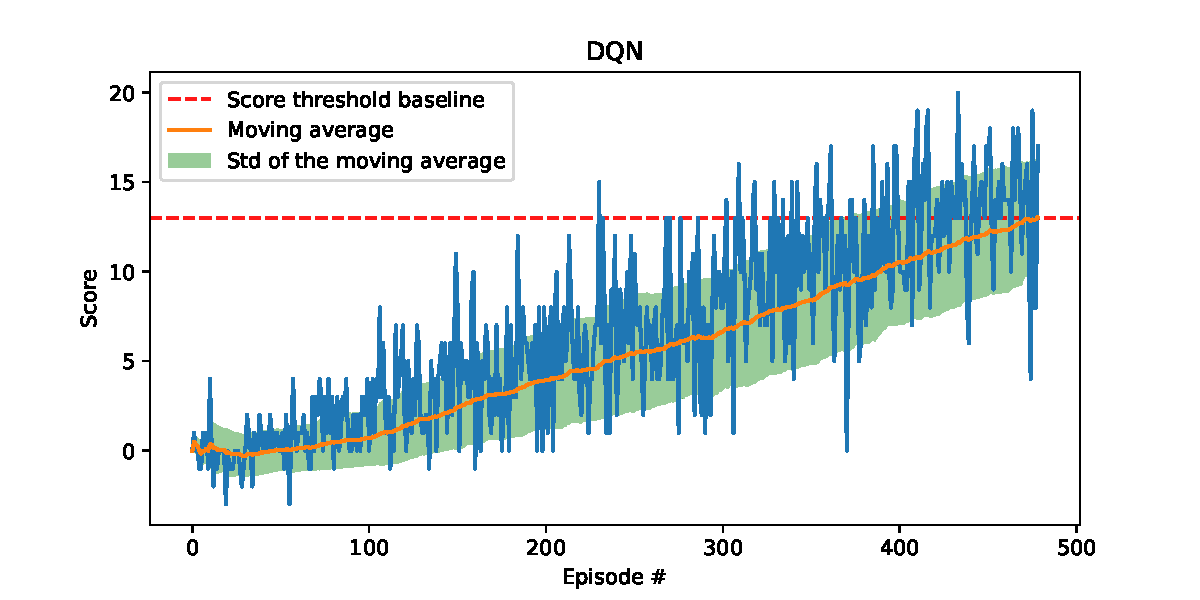
\includegraphics[width=\textwidth]{dqn_score}
        \caption{DQN}\label{fig:dqn}
    \end{subfigure}%
    ~ 
    \begin{subfigure}[t]{0.5\textwidth}
        \centering
        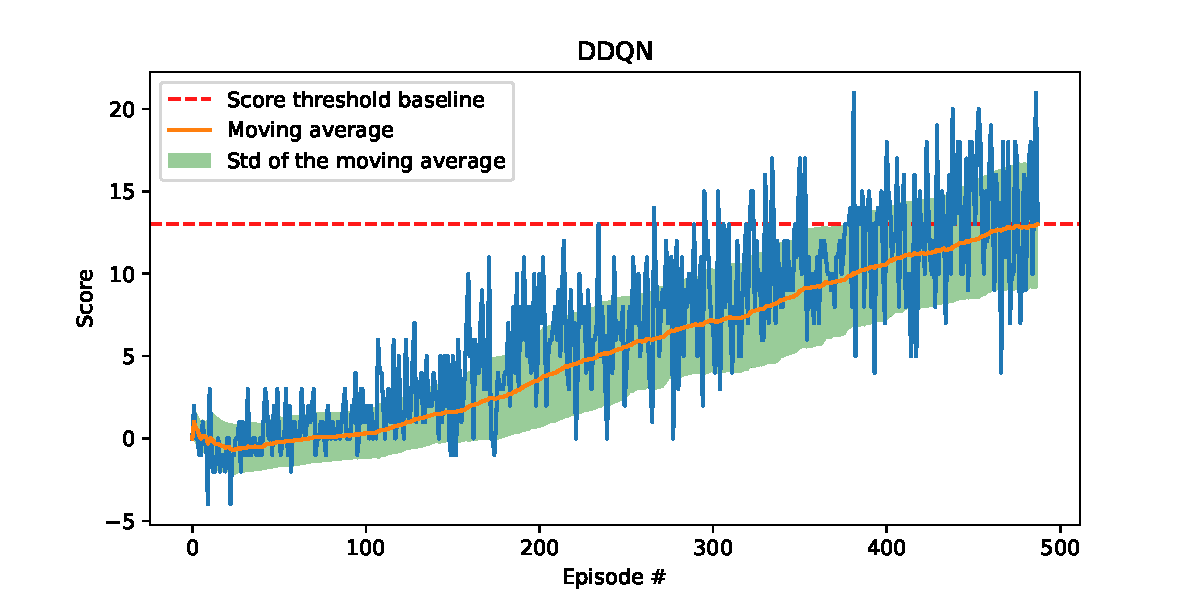
\includegraphics[width=\textwidth]{ddqn_score}
        \caption{DDQN}\label{fig:ddqn}
    \end{subfigure}
    \caption{Learning curves of DQN and DDQN algorithms}\label{fig:scores}
\end{figure*}

\bibliographystyle{IEEEtranN}%N enables \citeauthor and \citeyear in natbib, keeping the number format style.  
\bibliography{references}
\end{document}  